\chapter{Developer Guide}
\label{ch:developer}

\section{Libraries}

\subsection{NumPy}

NumPy stands for Numerical Python. It is a library used for scientific computing and it mainly deals with arrays and matrices. NumPy is written in Python, C, and C++ for fast computing. The size is fixed while creating NumPy arrays; therefore, a new array is created when the size is changed of the existing array and the original array is deleted. The elements in the NumPy array should have the same data type. Operations on large data in NumPy arrays are performed more efficiently and with less lines of code, that is why it is commonly used in data science, where speed and efficiency is very important \cite{numpy}.

We used NumPy in our project to help to clean data, to save cosine similarity matrix in npy file and load that npy file, so the algorithm did not have to be applied every time, we could save its results and load it.

Command to install Numpy: \texttt{pip install numpy}.

\subsection{Pandas}

Pandas is another python library. It is popular in data science. According to pandas documentation, it has powerful and flexible data structures which makes data analysis and manipulation easier.

There are two primary data structures in pandas:

\begin{itemize}
\item Series (1-dimensional);
\item DataFrame (2-dimensional).
\end{itemize}

Pandas is built on NumPy,  it can take a NumPy array 
and return a labeled index on the array.

Pandas Dataframe is actually a container of Pandas Series. Pandas Dataframe has three main components: data, index, and columns. DataFrame stores the data and to better classify it, we have the index that indicates the different rows and the column names that indicate the different columns. The index helps to fetch exact records \cite{pandas}.

We used Pandas DataFrame in our project to retrieve data in tabular form, clean and manipulate it.

Command to install pandas: \texttt{pip install pandas}.

\subsection{Matplotlib}

Matplotlib is a python library to plot graphs and visualizations. Matplotlib implements similar functionality to the plot features of matlab, but it has the advantage of being free and open-source \cite{matplotlib}. 

We used the Pyplot module in our project to plot histogram to visualize distributions. Pyplot has many functions like plotting figures, labeling and stylinzing them.

Command to install matplotlib: \texttt{pip install matplotlib}.

\subsection{Requests}

Requests is a python library, which helps to make HTTP requests to urls of web pages and fetch or post data.

We used this library in our project to get the movie's overview, duration and poster from omdb website using api.

Command to install requests: \texttt{pip install requests}.

\subsection{Scikit-learn}

Scikit-learn is another python library for Machine Learning algorithms like regression, classification, and clustering. This library is built upon the SciPy python library, SciPy is a python library for scientific computing.  Scikit-learn also combines with a lot other python libraries, such as NumPy for array vectorization, Pandas for dataframes, Matplotlib for plotting, and many more \cite{sk-learn}.

Scikit-learn is for modeling the data. Some of the models are: Clustering, Cross Validation, Feature Extraction, Feature Selection, Supervised and Unsupervised Learning algorithms \cite{sk-learn}.

We used the Feature selection model from scikit-learn library in our project to extract features in vector form and to compute distance matrix from feature vectors.

Command to install scikit-learn: \texttt{pip install scikit-learn}.

\subsection{Flask}

Web Server Gateway Interface (WSGI) describes the way of communication between a web server and web application and ties together the web applications to process one request.

Flask is one of popular python web application frameworks. It is a lightweight WSGI and micro framework. Here the word ‘micro’ means it points to keep the basic simple but extensible \cite{flask}.

Flask does not contain anything where different libraries already exist, a database abstraction layer, or form validation. It supports extensions to add for database integration, upload handling, form validation, and many more.

Command to install flask: \texttt{pip install Flask}.

\subsection{React}

React is a javascript library. It is used to build user interface components. The react project is created using node package manager (npm); which is Node.js package manager \cite{react-doc}. 

Command to create react project: \texttt{npm create-react-app (app name)} \cite{react-doc}.

Node.js is a javascript runtime environment which allows javascript to be used on a server. It is open source and runs on cross platforms.

Node package manager is installed with Node.js. It can manage dependencies and packages, which are defined in a json file named package.


\subsubsection{React Component}

React components allow to split the user interfaces into independent pieces that can be reused. It takes an optional parameter and returns the elements to be rendered on the screen.

There are two types of components:
\begin{itemize}
\item Stateful or Class component;
\item Stateless or Function component \cite{react-doc}.
\end{itemize}


\subsubsection{React Hooks}

React hooks are functions that allow the use of state and lifecycle features in function components without writing class components. They increase the code readability and decrease the use of class components. With hooks functional components handle state and logic rather than just rendering the user interface. Hooks can not be used inside if statements, nested function, loops and class components. Hooks can only be used inside functional components \cite{react-doc}.
 
There are 10 built-in hooks in react, we have only used two hooks in our project which are useState and useEffect. useState is used to handle and update the state in a function. It takes the initial state as an argument and returns two variables in the array. First variable is the current state and the second variable is a function which is used to update the state. useEffect is used to add side effects in function components. It takes effectual function and executes when the render is performed on the screen. By default effects are executed after each render, but there is an option to run them when some specific values change \cite{react-doc}. 


Semantic UI React is a user interface framework, which gives prebuilt react components and helps to build responsive and designable websites.

Command to install semantic ui react: \texttt{npm install semantic-ui-react semantic-ui-css} \cite{react-tutorial}.


\section{Model}

\subsection{Machine Learning}

Machine Learning (ML) is a part of artificial intelligence which has algorithms for creating models by learning from data and information. It implies computers to learn from provided data and perform certain tasks without being programmed explicitly \cite{ml-alpaydin}.

A major difference between human beings and machine learning has been for a long time that once a learning process is set into human minds, it is difficult to change it, but it is possible in machine learning by giving more data or changing the learning algorithms \cite{ml-janardhanan}. The human mind has limited capacity to learn and memorize things whereas machine learning algorithms process, learn and analyze huge amounts of data.

The term Machine Learning was given by a scientist Arthur Samuel in 1959. He created the world's first self-learning program called game of checkers which became better with the number of games it played \cite{ml-samuel}. The first pattern recognition algorithm was nearest neighbours to recognize patterns between new and known data \cite{ml-cover}. In the 1990s approach of knowledge driven was shifted to data driven in machine learning. Computer programs were created to analyze huge amounts of data and extract conclusions.


\subsection{Data Mining}

Data Mining is a subset of Machine Learning. It is a process to analyze large amounts of data and get knowledge from it. It also helps to find useful patterns and anomalies to get predictions from that data \cite{dm-iberdrola}. Data is growing rapidly, according to an international data corporation report prediction there will be 163 zettabytes of data by 2025 \cite{dm-idc}. We used similarity in our project for this, which is described later.

\subsection{Term Frequency}

Term Frequency (TF) is the computation of frequency of occurring words in a document. Since documents might differ in length, longer documents might have a bigger count of a certain word than shorter documents. Therefore, it is divided by the length of the document. i.e., the number of words in the document to normalize it \cite{Salton1983}.

\begin{equation}
TF (t) = \frac{\text{Number of times term t appears in a document}}{\text{Total number of terms in the document}}
\end{equation}

As an  example,  let us create a document containings a few movies from the 007 franchise to better understand the term frequency better. Each paragraph would be about one of the movies, but it would contain the features used in our recommendation system. As a remainder, the features are the genres, the main cast names, and the director’s name. The names are all lower case, and no space between first and last name.

Document: 

\begin{enumerate}
\item Casino Royale (2006)

Paragraph 1: "action adventure thriller judidench danielcraig jeffreywright evagreen martincampbell" 

\item Skyfall (2012)

Paragraph 2: "action adventure thriller javierbardem judidench danielcraig naomieharris sammendes" 

\item GoldenEye (1995)

Paragraph 3: "action adventure thriller piercebrosnan seanbean famkejanssen izabellascorupco martincampbell"
\end{enumerate}

There are a total 24 terms in this document, so the term frequency for these terms in the document would be following:

\begin{itemize}
\item action: 			3/24	=	0.125
\item adventure: 		3/24	=	0.125 
\item thriller: 			3/24	=	0.125
\item judidench: 		2/24	=	0.083
\item danielcraig: 		2/24	=	0.083
\item jeffreywright: 		1/24	=	0.041
\item evagreen: 		1/24	=	0.041
\item martincampbell: 	2/24	=	0.083
\item javierbardem: 		1/24	=	0.041
\item naomieharris: 		1/24	=	0.041
\item sammendes: 		1/24	=	0.041
\item piercebrosnan: 		1/24	=	0.041
\item seanbean: 		1/24	=	0.041
\item famkejanssen: 		1/24	=	0.041
\item izabellascorupco: 	1/24	=	0.041
\end{itemize}


\subsection{CountVectorizer}

CountVectorizer helps to convert text data to a vector of term counts. Vectorization is done by encoding words as integers or float values to use as input in machine learning algorithms. It returns the length of the word document and a count for the occurrences of each word in the document \cite{count-vectorizer}.

To continue the above example, we can vectorize the terms of the document.

\begin{blockarray}{cccccccccccccccc}
\centering
      & a & b & c & d & e & f & g & h & i & j & k & l & m & n & o \\
\begin{block}{c(ccccccccccccccc)}
  I   & 1 & 1 & 1 & 1 & 1 & 1 & 1 & 1 & 0 & 0 & 0 & 0 & 0 & 0 & 0 \\
  II  & 1 & 1 & 1 & 1 & 1 & 0 & 0 & 0 & 1 & 1 & 1 & 0 & 0 & 0 & 0 \\
  III & 1 & 1 & 1 & 0 & 0 & 0 & 0 & 1 & 0 & 0 & 0 & 1 & 1 & 1 & 1 \\ 
\end{block}
\end{blockarray}

In this table the row indexes 1, 2, and 3 represent the paragraphs numbers. The column indexes represents the terms, i.e

\begin{enumerate}[label=\alph*.]
\item action
\item adventure
\item thriller
\item judidench
\item danielcraig
\item jeffreywright
\item evagreen
\item martincampbell
\item javierbardem
\item naomieharris
\item sammendes
\item piercebrosnan
\item seanbean
\item famkejanssen
\item izabellascorupco
\end{enumerate}


\subsection{Cosine Similarity}

It computes by calculating the cosine of the angle between those two vectors. The vectors contain the word counts of the documents. If the cosine value is 1, it means the vectors are exactly similar and the angle between them is 0 degree. If the cosine value is 0, it means the vectors have no similarity between them and the angle is 90 degrees. If the cosine value is -1, then the vectors are exactly opposite of each other and the angle between them is 180 degrees. However, the last case does not happen in word count, since we just have positive integers for every dimension (word).  Smaller the angle between vectors the greater the similarity is between them.

Cosine similarity is expressed by

\begin{equation}
\cos \theta = \frac{X \cdot Y}{\mid X \mid \mid Y \mid} 
           = \frac{\sum_{i = 1}^{n}X_i Y_i}{\sqrt{\sum_{i = 1}^{n}X_i^2 \sum_{i = 1}^{n}Y_i^2}},
\end{equation}
where X and Y are term frequency vectors and Xi and Yi are components of the vectors. We take dot product of vectors and divide them by the product of the vectors' magnitude \cite{Han2017}.

Continuing the same example, we will now compute the cosine similarity among those movies.

First, between movie 1 and movie 2. We take dot product of term frequency vectors and divide by their magnitude.

\begin{equation*}
X = (1,1,1,1,1,1,1,1,0,0,0,0,0,0,0) \qquad Y = (1,1,1,1,1,0,0,0,1,1,1,0,0,0,0)
\end{equation*}
\begin{equation*}
X \cdot Y = \quad 1 \cdot 1 + 1 \cdot 1 + 1 \cdot 1 + 1 \cdot 1 + 1 \cdot 1 + 1 \cdot 0 + 1 \cdot 0 + 1 \cdot 0 + 0 \cdot 1 + 0 \cdot 1 + 0 \cdot 1 + 0 \cdot 0 + 0 \cdot 0 + 0 \cdot 0 + 0 \cdot 0 = 5
\end{equation*}
\begin{equation*}
\mid X \mid = \sqrt{1^2 + 1^2 + 1^2 + 1^2 + 1^2 + 1^2 + 1^2 + 1^2 + 0^2 + 0^2 + 0^2 + 0^2 + 0^2 + 0^2 + 0^2} = 2.828
\end{equation*}
\begin{equation*}
\mid Y \mid = \sqrt{1^2 + 1^2 + 1^2 + 1^2 + 1^2 + 0^2 + 0^2 + 0^2 + 1^2 + 1^2 + 1^2 + 0^2 + 0^2 + 0^2 + 0^2} = 2.828
\end{equation*}
\begin{equation}
\cos \theta = \frac{5}{2.828 \cdot 2.828} = 0.625
\end{equation}

Cosine similarity between movie 1 and movie 3 is 0.5.

The similarity between movie 1 and movie 2 is higher than between movie 1 and movie 3. This happens because in movie 1 and 2, there are 5 similar features, which are genres and two actors and in movie 1 and 3, there are 4 similar features, which are genres and the director.


\section{Backend}

\subsection{Datasets}

The datasets used in this project are from IMDb (Internet Movie Database)\footnote{\href{https://www.imdb.com/interfaces}{https://www.imdb.com/interfaces}}. We combined 6 basic datasets into one by analyzing, cleaning, and merging them.

From Title Basics, represented in Table \ref{tab:basics}, we need 5 attributes: (i) the unique movie id tconst as our index, (ii) the type titleType to filter only for movies, (iii) the title primaryTitle for the output of the recommendation , (iv) the movie release year startYear to also show in the output and to filter for recent movies, and (v) the genres genres to give as a feature to algorithm. 

\begin{table}[ht]
	\centering
	\caption{\textbf{Title Basics.} This dataset is a partial representation of Title Basics that contains the columns tconst, titleType, primaryTitle, startYear, genres.}
	\footnotesize
	\begin{tabular}{ccccc}
		\toprule
		tconst    & titleType & primaryTitle           & startYear & genres                     \\
		\midrule
		tt0000001 & short     & Carmencita             & 1894      & Documentary, Short         \\
		tt0000002 & short     & Le clown et ses chiens & 1892      & Animation, Short           \\
		tt0000003 & short     & Pauvre Pierrot         & 1892      & Animation, Comedy, Romance \\
		tt0000004 & short     & Un bon bock            & 1892      & Animation, Short           \\		
		tt0000005 & short     & Blacksmith Scene       & 1893      & Comedy, Short              \\
		$\cdots$  & $\cdots$  & $\cdots$               & $\cdots$  & $\cdots$                   \\
		\bottomrule
	\end{tabular}	
 	\label{tab:basics}
\end{table}

From Title Crew, shown in Table \ref{tab:crew}, we are using tconst for matching and directors to pass as a feature to the algorithm.

\begin{table}[ht]
	\centering
	\caption{\textbf{Title Crew.} This dataset is a partial of Title Crew representation that contains the columns tconst and directors.}
	\footnotesize
	\begin{tabular}{cc}
		\toprule
		tconst    & directors \\
		\midrule
		tt0000001 & nm0005690 \\
		tt0000002 & nm0721526 \\
		tt0000003 & nm0721526 \\
		tt0000004 & nm0721526 \\		
		tt0000005 & nm0005690 \\
		$\cdots$  & $\cdots$  \\
		\bottomrule
	\end{tabular}	
 	\label{tab:crew}
\end{table}

In Title Principals, as seen in Table \ref{tab:principals}, we are using 4 columns:  (i) the movie id tconst for matching, (ii) the order ordering that indicates the movie actors or cast number for each movie, (iii) the movie cast id for actors, actress, editor, etc nconst, and (v) the role category to better classify every cast.

\begin{table}[ht]
	\centering
	\caption{\textbf{Title Principals.} This dataset is a partial representation of Title Principals that contains the columns tconst, ordering, nconst, and category.}
	\footnotesize
	\begin{tabular}{cccc}
		\toprule
		tconst    & ordering & nconst    & category        \\
		\midrule
		tt0000001 & 1        & nm1588970 & self            \\
		tt0000001 & 2        & nm0005690 & director        \\
		tt0000001 & 3        & nm0374658 & cinematographer \\
		tt0000002 & 1        & nm0721526 & director        \\		
		tt0000002 & 2        & nm1335271 & composer        \\
		$\cdots$  & $\cdots$ &  $\cdots$ & $\cdots$        \\
		\bottomrule
	\end{tabular}	
 	\label{tab:principals}
\end{table}

In Title Ratings, represented in Table \ref{tab:ratings}, we collected the movie id tconst and the rating averageRating. We will use this rating and our algorithm score to define the raking by a weighted average.

\begin{table}[ht]
	\centering
	\caption{\textbf{Title Ratings.} This dataset is a partial representation of Title Ratings that contains the columns tconst and averagerating.}	
	\footnotesize
	\begin{tabular}{cc}
		\toprule
		tconst    & averageRating \\
		\midrule
		tt0000001 & 5.6           \\
		tt0000001 & 6.1           \\
		tt0000001 & 6.5           \\
		tt0000002 & 6.2           \\		
		tt0000002 & 6.2           \\
		$\cdots$  & $\cdots$      \\
		\bottomrule
	\end{tabular}	
 	\label{tab:ratings}
\end{table}

From Name Basics, as seen in Table \ref{tab:name}, we are only using the name id nconst and the actual name of the person primaryName. This dataset is to fetch the names of each crew member we have taken such as actors, actresses and directors.

\begin{table}[ht]
	\centering
	\caption{\textbf{Name Basics.} This dataset is a partial representation of Name Basics that contains the columns nconst and primaryName.}
	\footnotesize
	\begin{tabular}{cc}
		\toprule
		tconst    & averageRating   \\
		\midrule
		nm0000001 & Fred Astaire    \\
		nm0000002 & Lauren Bacall   \\
		nm0000003 & Brigitte Bardot \\
		nm0000004 & John Belushi    \\		
		nm0000005 & Ingmar Bergman  \\
		$\cdots$  &     $\cdots$    \\
		\bottomrule
	\end{tabular}	
 	\label{tab:name}
\end{table}

In Title AKAs, shown in Table \ref{tab:aka}, We took two columns: the movie id titleId and the region of the movie region. Because we wanted to fetch only American movies.

\begin{table}[ht]
	\centering
	\caption{\textbf{Title AKAs.} This dataset is a partial representation of Title AKAs that contains the columns titleId and region.}	
	\footnotesize
	\begin{tabular}{cc}
		\toprule
		titleId   & region   \\
		\midrule
		tt0000001 & UA       \\
		tt0000001 & DE       \\
		tt0000001 & HU       \\
		tt0000001 & GR       \\		
		tt0000001 & RU       \\
		$\cdots$  & $\cdots$ \\
		\bottomrule
	\end{tabular}	
 	\label{tab:aka}
\end{table}


\subsection{Data Pre-processing}

The first step was to filter only movies in Table \ref{tab:basics}, as there are TV shows and short movies as well and we saved the results in the same pandas DataFrame.

\begin{lstlisting}[language=python]
basics_df.query("titleType == 'movie'", inplace=True)
\end{lstlisting}

Next, we filtered actors and actresses from the Title Principals (Table \ref{tab:principals}), as there are also other crew members, such as, producer, cameraman, and etc. Again, we stored the result in the same variable.

\begin{lstlisting}[language=python]
principals_df.query("category in ['actor', 'actress']", inplace=True)
\end{lstlisting}

We also add a filter for the US region, as there are many other regions like FR, HU, JP, and etc. Our system is focused only in American movies. Once more, we replace the result in the original dataset.

\begin{lstlisting}[language=python]
titles_info_df.query("region in ['US']", inplace=True)
\end{lstlisting}

Now, we can finally merge some of the results. The first merge is Names Basics (Table \ref{tab:name}),  where all the crew member names and ids are stored,  and Title Principals (Table \ref{tab:crew}), where director ids are stored. It is performed on the columns 'nconst' and 'directors' by applying an inner join, which takes the intersection of ids. We also renamed the column name from 'primaryName' to 'directorName' and stored only the movie id ('tconst') and director's name. The result was saved in a new DataFrame.

\begin{lstlisting}[language=python]
directors_df=pd.merge(names_df,crew_df,left_on='nconst',right_on='directors',how='inner')
directors_df = directors_df.rename(columns={'primaryName':'directorName'})
directors_df= directors_df[['tconst','directorName']]
\end{lstlisting}

The next merge was Name Basics (Table \ref{tab:name}), where all the crew member names and ids are stored, and Title Principals (Table \ref{tab:principals}), where actors and actress ids are stored for each movie. We also did an inner join on 'nconst' columns. We also renamed the name of column 'primaryName' to 'actorName' and stored it in a new dataframe.

\begin{lstlisting}[language=python]
cast_df= pd.merge(names_df,principals_df,on='nconst',how='inner')
cast_df = cast_df.rename(columns={'primaryName':'actorName'})
\end{lstlisting}

We kept working on the same DataFrame to select the actors/actresses of each movie, and stored it in a new dataframe. Later we dropped the duplicate tconst.

\begin{lstlisting}[language=python]
actor_df = cast_df.groupby('tconst')['actorName'].apply(', '.join).reset_index()
actor_df.drop_duplicates(subset=['tconst'], inplace=True)
\end{lstlisting}

Now we are going to separate and rename the important information from Title Basics (Table \ref{tab:basics}). 

\begin{lstlisting}[language=python]
basics_df = basics_df[['tconst','primaryTitle','startYear','genres']]
basics_df = basics_df.rename(columns={'primaryTitle':'title', 'startYear':'year'})
\end{lstlisting}

We removed the 0's from every column in the dataFrame, because there were '\\N' in dataFrame initially, so we manually replaced '\\N' with '0's. We are also focusing on recent movies, so a filter is made to select movies which are released after 1990. We added space between genres and also removed the movies which have '?' in the end of their title, because they were duplicates.

\begin{lstlisting}[language=python]
basics_df= basics_df.query("tconst != '0'")
basics_df=basics_df.query("title != '0'")
basics_df=basics_df.query("year != 0")
basics_df=basics_df.query("genres != '0'")

basics_df=basics_df.query("year > 1990")
basics_df['genres'] = basics_df['genres'].str.replace(',', ', ')
indices = basics_df['title'][basics_df['title'].str.endswith("?")].index
basics_df.drop(indices, inplace=True)
\end{lstlisting}

To have some better insights about the rating, we can plot the distribution of the average rating by the pyplot method from matplotlib.  As seen in Figure \ref{fig:graph}.

\begin{lstlisting}[language=python]
import matplotlib.pyplot as plt
%matplotlib inline

plt.figure(figsize =(10, 4))   
ratings_df['averageRating'].hist(bins = 10)
plt.xlabel('averageRating')
plt.ylabel('Count')
plt.title(r'average rating distribution')
\end{lstlisting}

\begin{figure}[ht]
	\centering
  	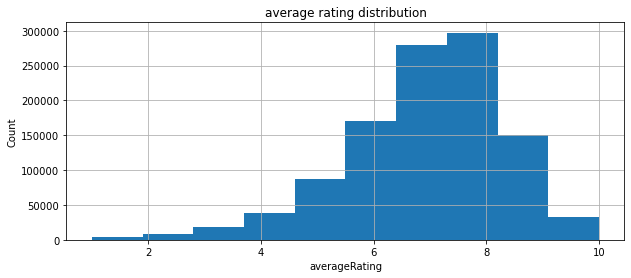
\includegraphics[width=0.8\textwidth]{images/graph.png}
	\caption{\textbf{Graph of Rating Distribution.}This figure is a visual distribution of average rating.}
  	\label{fig:graph}
\end{figure}


To organize the dataset, more renaming was done. To prepare it for the algorithm.

\begin{lstlisting}[language=python]
actor_df = actor_df.rename(columns={'actorName':'actors'})
directors_df = directors_df.rename(columns={'directorName':'director'})
ratings_df = ratings_df.rename(columns={'averageRating':'rating'})
\end{lstlisting}

We can finally merge all the information together with an inner join on 'tconst'. We called this new variable as final\_movies\_df. 

\begin{lstlisting}[language=python]
final_movies_df=pd.merge(basics_df,actor_df,on='tconst',how='inner')
.merge(directors_df,on='tconst',how='inner')
.merge(ratings_df,on='tconst',how='inner')
.merge(titles_info_df,on='tconst',how='inner')
\end{lstlisting}

Again, to better feed the algorithm, we added a new column 'combine' which contains all our feature columns which are genres, actor names, and director names.

\begin{lstlisting}[language=python]
final_movies_df['combine']= final_movies_df['genres']+","+final_movies_df['actors']+","+final_movies_df['director']
\end{lstlisting}

To further clean up, we removed duplicates from movie ids and movie titles and stored them in the same dataframe which is final\_movies\_df.

\begin{lstlisting}[language=python]
final_movies_df.drop_duplicates(subset='tconst', keep="first", inplace=True)
final_movies_df.drop_duplicates(subset='title', keep="first", inplace=True)
\end{lstlisting}

We did another treatment to the combine column using the function names\_together\_lower. This function takes the column as a parameter and converts all letters into lower case and then removes the spaces between first name and last name of actors and directors, e.g. 'Chris Hemsworth' as 'chrishemsworth' and 'Chris Evans' as 'chrisevans'. Otherwise the algorithm would match Chris in both names and it would not be accurate. Later this function replaces commas with space between our all features. The result is saved in another column called combined.

\begin{lstlisting}[language=python]
def names_together_lower(x):
    x=np.char.lower(x)
    x=np.char.replace(x," ", "")
    x=np.char.replace(x,","," ")
    return x

final_movies_df['combined']=final_movies_df['combine'].apply(names_together_lower)
\end{lstlisting}

Now we do not need 'region' and 'combine'. We have already fetched English movies and stored our features in the 'combined' column. 

\begin{lstlisting}[language=python]
final_movies_df.drop(['region'], axis = 1, inplace=True) 
final_movies_df.drop('combine', inplace=True, axis=1)
\end{lstlisting}

The last step of the cleaning was to reset the index of the DataFrame and save the final dataframe as Final\_MovieData in pickle and csv format.

\begin{lstlisting}[language=python]
final_movies_df.reset_index(drop=True, inplace=True)

final_movies_df.to_pickle('Final_MovieData.pkl')
final_movies_df.to_csv('Final_MovieData.csv')
\end{lstlisting}


\subsection{Data Modeling}

We first need to import the necessary libraries as:
\begin{itemize}
\item Pandas with alias pd
\item Numpy with alias np
\item Requests to get data from OMDB api.
\item From the flask library it imports Flask to instantiate the flask app,  request to get requests from clients, and jsonify to fetch and return json files.
\item From the scikit learn feature extraction it imports CountVectorizer to create our text format feature into numerical matrix computing term frequency.
\item From scikit learn metrics pairwise it imports cosine\_similarity algorithm to apply on our matrix and get the similar recommendation.
\end{itemize}


\begin{lstlisting}[language=python]
import pandas as pd
import numpy as np
from flask import Flask, request, jsonify
from sklearn.feature_extraction.text import CountVectorizer
from sklearn.metrics.pairwise import cosine_similarity
\end{lstlisting}

Now we load our data which as previously cleaned, the code reads the csv file which is our final dataset (Table \ref{tab:final}) and stores it in the movies variable.

\begin{lstlisting}[language=python]
movies = pd.read_csv('Final_MovieData.csv')
\end{lstlisting}

\begin{table}[ht]
	\centering
	\caption{\textbf{Final Movie Dataset.} This dataset is a partial representation of the Final Movie dataset that contains the columns index, tconst, title, year, rating, and combined.}	
	\footnotesize
	\begin{tabular}{cccccc}
		\toprule
		index    & tconst    & title                         & year     & rating   & combined           \\
		\midrule
		0        & tt0035425 & Kate \& Leopold               & 2001     & 6.4      & comedy fantasy     \\
		         &           &                               &          &          & romance megryan    \\
		         &           &                               &          &          & hughjackman        \\
		         &           &                               &          &          & lievschreiber      \\
		         &           &                               &          &          & jamesmangold       \\
		1        & tt0064730 & Japan Organization Crime Boss & 2000     & 7.0      & action crime       \\
		         &           &                               &          &          & kôjitsuruta        \\
		         &           &                               &          &          & tomisaburôwakayama \\
		         &           &                               &          &          & buntasugawara      \\
		         &           &                               &          &          & kinjifkasaku       \\
		2        & tt0069049 & The Other Side of the Wind    & 2018     & 6.8      & drama johnhuston   \\
		         &           &                               &          &          & ojakodar           \\
		         &           &                               &          &          & peterbogdanovich   \\ 
		         &           &                               &          &          & orsonwelles        \\
		3        & tt0081145 & Me and the Kid                & 1993     & 5.4      & comedy crime drama \\
		         &           &                               &          &          & dannyaiello        \\ 
		         &           &                               &          &          & alexzuckerman      \\
		         &           &                               &          &          & joepantoliano      \\
		         &           &                               &          &          & dancurtis          \\
		4        & tt0094900 & Committed                     & 1991     & 5.1      & drama thriller     \\
		         &           &                               &          &          & jennifero’neill    \\ 
		         &           &                               &          &          & robertforster      \\
		         &           &                               &          &          & williamwindom      \\
		         &           &                               &          &          & williams.levey     \\
		$\cdots$ & $\cdots$  & $\cdots$                      & $\cdots$ & $\cdots$ & $\cdots$           \\
		\bottomrule
	\end{tabular}	
 	\label{tab:final}
\end{table}

This is our final data which we are using for our recommendation system which has movie id, movie title, released year of the movie, user average rating and feature column combine which contains all the features like genres, actor names, and director. This feature column will be passed to algorithm to get recommendations.

Following function takes imdb\_id as a parameter and fetches movie duration time, overview and poster from omdb api website, which is a public api for imdb movies. We request by our api key and imdb\_id and get a response in json format. If the data is not available for some specific movies on that api then we set the default values for that. We return a dictionary with data.

\begin{lstlisting}[language=python]
def get_imdb_data(imdb_id):
   basic_url = "http://www.omdbapi.com/"
   api_key = "fc796b50"
   response_data = requests.get(f"{basic_url}?apikey={api_key}&i={imdb_id}").json()
   runtime = response_data['Runtime']
   if runtime == 'N/A':
       runtime = 'min N/A'
   plot = response_data['Plot']
   if plot == 'N/A':
       plot = 'Overview: Not Available'
   poster = response_data['Poster']
   if poster == 'N/A':
       poster = "https://i.postimg.cc/Vk6xs9K8/default.jpg"
   imdb_data = {
       'run_time': runtime,
       'overview': plot,
       'poster': poster
   }
   return imdb_data
\end{lstlisting}

The next function takes index of a movie as a parameter and gets movie title, year, movie id, rating, and genre from dataset and calls the get\_imdb\_data function on tconst to fetch movie runtime, overview and poster and returns all this data as a dictionary.

\begin{lstlisting}[language=python]
def get_user_searched_movie(ind):
   title = movies.loc[ind, 'title']
   year = int(movies.loc[ind, 'year'])
   imdb_id = movies.loc[ind, 'tconst']
   rating = movies.loc[ind, 'rating']
   genres = movies.loc[ind, 'genres']
   imdb_data = get_imdb_data(imdb_id)
   runtime = imdb_data['run_time']
   overview = imdb_data['overview']
   poster = imdb_data['poster']
   searched_movie_data = {
       'id': 1,
       'title': title,
       'year': year,
       'genres': genres,
       'rating': rating,
       'runtime': runtime,
       'overview': overview,
       'poster': poster
   }
   return searched_movie_data
\end{lstlisting}

The function update\_matrix creates the instance of CountVectorizer class and learns the vocabulary and encodes it into a matrix. Then it saves that matrix locally as a npy file and if any error occurs while computing the similarity matrix, it prints the error. 

\begin{lstlisting}[language=python]
def update_matrix():
   try:
       cv = CountVectorizer(dtype=np.float32)
       movie_matrix = cv.fit_transform(movies['combined'])
       cos_similarity = cosine_similarity(movie_matrix)
       np.save('cosine_matrix.npy', cos_similarity)
   except:
       print("There was some error while updating the matrix")
\end{lstlisting}

To load the cosine similarity matrix file, we simply used numpy to store it in the cos\_s variable. We are saving and loading this file because of memory issue, computing cosine similarity on this large dataset consumes a lot of memory. So we save this file locally once and then we load every time to get the recommendations. It is also static, so we can cache the information instead of calculating every time.

\begin{lstlisting}[language=python]
cos_s = np.load('cosine_matrix.npy')
\end{lstlisting}

get\_cosine\_scores takes index of the movie as a parameter, collects the cosine similarity score and stores in the list of tuples which contains index and cosine score of movies.  Afterwards, it is sorted in descending order according to the cosine score which means the movie that has a high similar score comes first. We return a list of indexes of the similar movies and similarity scores of top 50 movies. 

\begin{lstlisting}[language=python]
def get_cosine_scores(ind):
   similarity_scores = list(enumerate(cos_s[ind]))
   similarity_scores = sorted(similarity_scores, key=lambda x: x[1], reverse=True)
   similarity_scores = similarity_scores[1:51] 
   return similarity_scores
\end{lstlisting}

The next function takes a list of indexes of the similar movies and cosine similarity score as a parameter.  It iterates through all the indexes and scores and stores all the ratings from the dataset (Table 7) in a variable with respect to indexes. Then it takes the weighted average of similarity score and user rating by ratio 2:1 using the equation (1) for each index

\begin{equation}
\frac{2 \cdot \text{score} + \text{rating}/10}{3},
\label{eq:average}
\end{equation}
where, we divide the rating by 10 so that both score and rating are between 0 and 1.

\begin{lstlisting}[language=python]
def weight_average_cosineScore_rating(cos_scores):
   averages = []
   for i, score in cos_scores:
       rating = movies.loc[i, 'rating']
       average = (2 * score + (rating / 10)) / 3
       averages.append((i, average))
   averages = sorted(averages, key=lambda x: x[1], reverse=True)
   averages = averages[0:10]
   indexes = list(map(lambda item: item[0], averages))
   return indexes
\end{lstlisting}

Later we add the indexes and weighted average into a list, and we sort that list in descending order according to the average score which means the movie that has the highest average comes first. Then, we take the top 10 out of that list and only return the list of movie indexes.

Following function takes the list of movie indexes as a parameter. It iterates through the list and takes title, year and imdb\_id of the movie from dataframe (Table \ref{tab:final}) and calls get\_imdb\_data function to fetch a poster for each movie from omdb api. Afterwards, it stores all the information in variables. After that it adds  id, which is generated through a loop from 1 to 10, title, year and poster in a list as a dictionary and returns that list.

\begin{lstlisting}[language=python]
def get_movies_data(ind):
   movies_data = []
   j = 1
   for i in ind:
       title = movies.loc[i, 'title']
       year = int(movies.loc[i, 'year'])
       imdb_id = movies.loc[i, 'tconst']
       poster = get_imdb_data(imdb_id)['poster']
       movies_data.append({'id': j, 'title': title, 'year': year, 'poster': poster})
       j = j + 1
   return movies_data
\end{lstlisting}

The recommendations function is our main function which takes the movie title from the user as a parameter and checks if it is unique. Later it calls all the above functions. First, it calls the indexes series which returns the index of the movie which is given as a parameter, then it calls get\_user\_searched\_movie function to get all the information about the searched movie. Later it calls get\_cosine\_scores function with that index to calculate similarity score for similar movies and returns a list of top 50 cosine scores and their indexes. After that weight\_average\_cosineScore\_rating function is called which calculates weighted average and returns top 10 movie indexes calculated based on weighted average of cosine score and user rating. Finally the get\_movies\_data function is called by giving a list of indexes as a parameter to fetch movie names, movie released year and movie poster in a variable. This function returns a list of 2 dictionaries with user searched movie data and recommended movies, if the user searched movie is in our dataframe. Otherwise, it returns the message that this movie is not in our database.

\begin{lstlisting}[language=python]
def recommendations(title):
   return_movies_data = []
   if title in movies['title'].unique():
       index = indexes[title]
       user_searched_movie = get_user_searched_movie(index)
       records = get_cosine_scores(index)
       records = weight_average_cosineScore_rating(records)
       records = get_movies_data(records)
       um = {
           'user_searched_movie_data': user_searched_movie
       }
       rm = {
           'recommended_movies': records
       }
       return_movies_data.append(um)
       return_movies_data.append(rm)
       return return_movies_data
\end{lstlisting}

To create the web app an instance of class Flask is created with two endpoints and their route decorators. Route decorator is used to trigger the function to be called by telling the url to flask app. By default the HTTP method is 'GET', but to give other methods we need to specify them in route decorator with methods variable. We have only used the 'POST' method in our project, so if the incoming request is 'Post', then the functions take the movie name in json format given by user and store it in movie\_name variable and call the recommendations function on that movie name. Recommendations function returns the id, movie title, and year in a list and then it is returned in a json format by using the jsonify function. Function for url recommendations is called when the user type a movie name in search bar, and function for url clickRecommendations is called when user clicks on one of the previously recommended movies to get recommendations. 

\begin{lstlisting}[language=python]
app = Flask(__name__)

@app.route('/recommend', methods=['POST'])
def recommend():
   if request.method == 'POST':
       data = request.get_json()
       movie_name = data['title']
       rec = recommendations(movie_name)
       return jsonify({'movies': rec})

@app.route('/clickRecommendations', methods=['POST'])
def clickRecommendations():
   if request.method == 'POST':
       data = request.get_json()
       movie_name = data
       rec = recommendations(movie_name)
       return jsonify({'clickedMovies': rec, 'title': movie_name})

if __name__ == '__main__':
   app.run(debug=True)
\end{lstlisting}


\section{Frontend}

We use React for frontend design. We have two components. One is the form component to get a movie name from the user and fetch a recommend end point and another one is to show details of a searched movie and list recommended movies. We call these both components in main which is app.js. We also change the background every 10 seconds.

The following component imports react and useState hook from react and semantic ui components. It creates a form with two form fields which are input and a button. Input field is for the user to type the movie name in it and we store that value in title useState.  When the user clicks the button, the api call to recommend endpoint is initiated and user typed input is sent to backend in json and then response is received from backend in json. In response, we get details for the user searched movie and top 10 movie recommendations and the input field is set to empty.

\begin{lstlisting}[language=HTML]
import React, { useState } from "react";
import { Form, Input, Button } from "semantic-ui-react";
 
export const RecommendationForm = ({ onMovies, onCurrentMovie }) => {
    const [title, setTitle] = useState("");
 
    return (
        <Form className="movie-form">
            <Form.Field className="search-field">
                <Input id="inputfield"
                    icon={{ name: "search", circular: true, link: true }}
                    placeholder="Get Movie Recommendations. Search here..."
                    value={title}
                    onChange={(e) => setTitle(e.target.value)}
                />
            </Form.Field>
            <Form.Field className="searchbt">
                <Button
                    id="click-search"
                    onClick={async () => {
                        const movie = { title };
                        fetch("/recommend", {
                            method: "POST",
                            headers: {
                                "Content-Type": "application/json",
                            },
                            body: JSON.stringify(movie),
                        })
                            .then((response) => response.json())
                            .then((data) => {
                                onMovies(data.movies[1].recommended_movies);
                                onCurrentMovie(data.movies[0].user_searched_movie_data);
                                setTitle("");
                            });
                    }}
                >
                    Search
                </Button>
            </Form.Field>
        </Form>
    );
};
\end{lstlisting}

The next component first checks the response from the backend, if the user searched movie id is 0 in response, then it shows the message that this movie does not exist in our database. Otherwise it shows the details of the searched movie which is name, released year, poster, rating, genres, running time, and overview. It also shows the list of recommended movies with name, year and poster. After getting recommendations, if the user clicks over one of the recommended movies, it calls the clickRecommendations endpoint with clicked movie title and gets response with the details and the recommendations according to that clicked movie. 

\begin{lstlisting}[language=HTML]
export const ListMovies = ({
    recommendedMovies,
    currentMovie,
    clickedRecommendedMovies,
    clickedCurrentMovie,
}) => {
    return (
        <div className="movie-list">
            <div className={currentMovie.id === undefined ? "unactive" : "active"}>
                <div className={currentMovie.id === 0 ? "null-movie" : "current-movie-null"}>
                    <h1>The movie you are trying to search is not available.</h1>
                </div>
                <div className= {currentMovie.id === 0 ? "current-movie-null" : "current-movie"}>
                    <img className="poster" src={currentMovie.poster} alt="poster"></img>
                    <div className="movie-details">
                        <span className="title">{currentMovie.title}</span>
                        <span>({currentMovie.year})</span>
                        <div className="runtime-genres">
                            <span>
                                {currentMovie.runtime} | {currentMovie.genres}
                            </span>
                        </div>
                        <div className="rating">
                            <span className="star">&#x2605;</span>
                            <span>{currentMovie.rating}/10</span>
                        </div>
                        <span className="overview">{currentMovie.overview}</span>
                    </div>
                </div>
                <div className={currentMovie.id === 0 ? "current-movie-null" : "title-recommended-movies"}> Recommended Movies for you: </div>
            </div>
            <div className={currentMovie.id === 0 ? "current-movie-null" : "list-of-movies"}>
                {recommendedMovies.map((movie) => {
                    return (
                        <div className="movies" key={movie.id}>
                            <div
                                onClick={async () => {
                                    fetch("/clickRecommendations", {
                                        method: "POST",
                                        headers: {
                                            "Content-Type": "application/json",
                                        },
                                        body: JSON.stringify(movie.title),
                                    })
                                        .then((response) => response.json())
                                        .then((data) => {
                                            clickedRecommendedMovies(data.clickedMovies[1].recommended_movies);
                                            clickedCurrentMovie(data.clickedMovies[0].user_searched_movie_data);
                                        });
                                }}
                            >
                                <div className="recomended-movies">
                                    <img
                                        className="poster-recommend"
                                        src={movie.poster}
                                        alt="poster"
                                    ></img>
                                    <div className="movie-details-recomended">
                                        <span className="title title-recomended">{movie.title}</span>
                                        <span>({movie.year})</span>
                                    </div>
                                </div>
                            </div>
                        </div>
                    );
                })}
            </div>
        </div>
    );
};
\end{lstlisting}

We call both components in the App.js file. Component RecommendationForm is given two functions as parameters to get user searched movie details and recommended movies, and component ListMovies is given two variables to show user searched movie details and recommended movies and two functions to get the details and recommended movies for one of the recommended movies as parameters. We also change the background image every 10 seconds. 

\begin{lstlisting}[language=HTML]
import React, { useState, useEffect } from "react";
import "./App.css";
import { ListMovies } from "./components/ListMovies";
import { RecommendationForm } from "./components/RecommendationForm";
 
function App() {
    const [recommendedMovies, setRecommendedMovies] = useState([]);
    const [currentMovie, setCurrentMovie] = useState([]);
    const [url, setUrl] = useState(["", "/static/media/857752.7ac2bde8.png"]);
 
<h1 className="project-title">Movie Recommendation System</h1>
            <RecommendationForm onMovies={(movie) => setRecommendedMovies(movie)} onCurrentMovie={(movie) => setCurrentMovie(movie)} />
            <ListMovies
                className="movie-component"
                recommendedMovies={recommendedMovies}
                currentMovie = {currentMovie}
                clickedRecommendedMovies={(movie) => setRecommendedMovies(movie)}
                clickedCurrentMovie ={(movie) => setCurrentMovie(movie)}
            />}
export default App;
\end{lstlisting}

\section{Example}

In (Table \ref{tab:comparison}) let's compare the movies ranking with weighted average of rating and cosine score like in \eqref{eq:average} and just cosine score. Taking movie Casino Royale from the above example and compare the top 15 recommendations.

\begin{table}[ht]
	\centering
	\caption{\textbf{Comparison between movie positions.} This table shows the comparison between recommending movies based on cosine score and based on average of cosine score and user rating.}	
	\footnotesize
	\begin{tabular}{c|cc|cccc}
	\toprule
	         & \multicolumn{2}{c|}{Without Rating} & \multicolumn{4}{c}{With Rating}                \\
	\midrule
	         &                      & Cosine &                         & Cosine &        & Weighted \\
	Position & Movie Name           & Score  & Movie Name              & Score  & Rating & Average  \\
	\midrule
	1        & Quantum of Solace    & 0.625  & Skyfall                 & 0.625  & 7.7    & 0.673    \\
	2        & Skyfall              & 0.625  & Quantum of Solace       & 0.625  & 6.6    & 0.636    \\
	3        & GoldenEye            & 0.5    & GoldenEye               & 0.5    & 7.2    & 0.573    \\
	4        & Spectre              & 0.5    & Spectre                 & 0.5    & 6.8    & 0.559    \\
	5        & CIA Code Name: Alexa & 0.375  & The Rock                & 0.375  & 7.4    & 0.496    \\
	6        & Hard Hunted          & 0.375  & Low Heights             & 0.375  & 7.4    & 0.496    \\
	7        & Cliffhanger          & 0.375  & Mission: Impossible -   & 0.375  & 7.4    & 0.496    \\
	         &                      &        & Ghost Protocol          &        &        &          \\
	8        & Angel of Destruction & 0.375  & Mission: Impossible -   & 0.375  & 7.4    & 0.496    \\
	         &                      &        & Rogue Nation            &        &        &          \\
	9        & Drop Zone            & 0.375  & The Adventures of       & 0.375  & 7.3    & 0.493    \\
	         &                      &        & Tintin                  &        &        &          \\
	10       & Speed                & 0.375  & Speed                   & 0.375  & 7.2    & 0.489    \\
	11       & Breakaway            & 0.375  & Kingdom of Heaven       & 0.375  & 7.2    & 0.489    \\
	12       & Broken Arrow         & 0.375  & Mission: Impossible     & 0.375  & 7.1    & 0.486    \\
	13       & Executive Decision   & 0.375  & Fast \& Furious 6       & 0.375  & 7.1    & 0.486    \\
	14       & Mission: Impossible  & 0.375  & Death Proof             & 0.375  & 7.0    & 0.483    \\
	15       & The Rock             & 0.375  & Mission: Impossible III & 0.375  & 6.9    & 0.479    \\
	\bottomrule
	\end{tabular}	
 	\label{tab:comparison}
\end{table}

As we can see that the first four movies are from 007 franchise but 1st and 2nd movie exchange their position which can be seen that Skyfall has better user ranking than Quantum of Solace. With a weighted average we get similar action and adventure movies as casino royale. In the table many movies have the same cosine similarity score, but after combining with rating the better movies come up. For example The Rock movie is on position 15 without rating, but after it is on position 5.





